\documentclass{article}
\usepackage{amsmath}
\usepackage{listings}
\usepackage{xcolor}
\usepackage{graphicx}
\usepackage{geometry}
\usepackage{hyperref}
\usepackage{tikz}
\usetikzlibrary{trees, positioning}
\geometry{margin=1in}

\title{Recursive backtracking}
\author{}
\date{}

\definecolor{codegray}{rgb}{0.5,0.5,0.5}
\definecolor{backcolour}{rgb}{0.95,0.95,0.92}

\lstdefinestyle{cppstyle}{
  backgroundcolor=\color{backcolour},
  commentstyle=\color{codegray},
  keywordstyle=\color{blue},
  numberstyle=\tiny\color{codegray},
  stringstyle=\color{red},
  basicstyle=\ttfamily\footnotesize,
  breakatwhitespace=false,
  breaklines=true,
  captionpos=b,
  keepspaces=true,
  numbers=none,
  numbersep=5pt,
  showspaces=false,
  showstringspaces=false,
  showtabs=false,
  tabsize=2,
  language=C++
}

\begin{document}

\maketitle



\section{What is Recursive Backtracking?}
Recursive backtracking uses recursion to explore solutions and abandons (backtracks) partial solutions when they fail.

Goals:
\begin{itemize}
  \item Determine whether a solution exists
  \item Find a solution
  \item Find the best solution
  \item Count the number of solutions
  \item Print or find all solutions
\end{itemize}

Applications:
\begin{itemize}
  \item Puzzle solving (e.g. Sudoku, crosswords)
  \item Game playing (e.g. Chess, solitaire)
  \item Constraint satisfaction (e.g. scheduling, matching)
\end{itemize}

\section{The Recursion Checklist}
\begin{itemize}
  \item What information do we track?
  \item What is the base case?
  \item What is the recursive step?
  \item Are all inputs handled?
\end{itemize}

\section{The Backtracking Checklist}
\begin{itemize}
  \item What are our choices at each step?
  \item Make a choice and recurse
  \item Undo the choice
  \item What happens at the base case?
\end{itemize}

---

\section{Example: printAllBinary}

\begin{center}
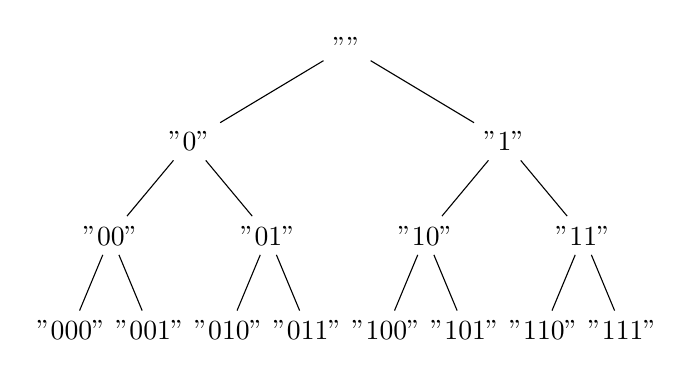
\begin{tikzpicture}[level distance=1.2cm,
  level 1/.style={sibling distance=4cm},
  level 2/.style={sibling distance=2cm},
  level 3/.style={sibling distance=1cm}]
\node {""}
  child {node {"0"}
    child {node {"00"}
      child {node {"000"}}
      child {node {"001"}}
    }
    child {node {"01"}
      child {node {"010"}}
      child {node {"011"}}
    }
  }
  child {node {"1"}
    child {node {"10"}
      child {node {"100"}}
      child {node {"101"}}
    }
    child {node {"11"}
      child {node {"110"}}
      child {node {"111"}}
    }
  };
\end{tikzpicture}
\end{center}

\begin{lstlisting}[style=cppstyle]
void printAllBinary(int numDigits) {
    printAllBinaryHelper(numDigits, "");
}

void printAllBinaryHelper(int digits, string soFar) {
    if (digits == 0) {
        cout << soFar << endl;
    } else {
        printAllBinaryHelper(digits - 1, soFar + "0");
        printAllBinaryHelper(digits - 1, soFar + "1");
    }
}
\end{lstlisting}

\section{Example: Dice Rolls}

The dice rolls problem asks us to generate and print all possible sequences of rolls of a given number of dice, where each die has 6 sides. This is a classic recursive backtracking problem where:
\begin{itemize}
    \item Each recursive call represents choosing a value for one die.
    \item We explore all possibilities by trying values 1 through 6 at each level of recursion.
    \item After exploring, we backtrack by undoing the choice to try alternatives.
\end{itemize}

The total number of sequences for rolling $n$ dice is $6^n$.

\subsection*{Code for Dice Rolls}

\begin{lstlisting}[style=cppstyle]
void diceRolls(int dice) {
    Vector<int> chosen;
    diceRollHelper(dice, chosen);
}

void diceRollHelper(int dice, Vector<int>& chosen) {
    if (dice == 0) {
        cout << chosen << endl;
    } else {
        for (int i = 1; i <= 6; i++) {
            chosen.add(i);
            diceRollHelper(dice - 1, chosen);
            chosen.remove(chosen.size() - 1);
        }
    }
}
\end{lstlisting}

\textbf{Call tree (2 digits):}

\begin{center}
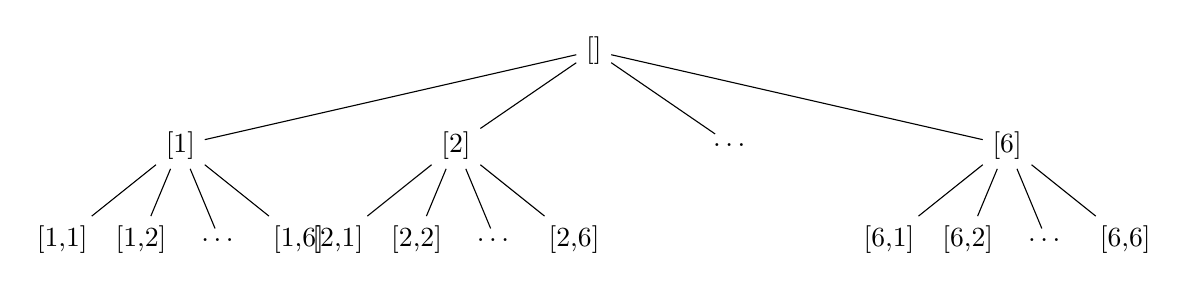
\begin{tikzpicture}[
  level 1/.style={sibling distance=3.5cm},
  level 2/.style={sibling distance=1cm},
  level distance=1.2cm
]
\node {[]}
  child {node {[1]}
    child {node {[1,1]}}
    child {node {[1,2]}}
    child {node {\dots}}
    child {node {[1,6]}}
  }
  child {node {[2]}
    child {node {[2,1]}}
    child {node {[2,2]}}
    child {node {\dots}}
    child {node {[2,6]}}
  }
  child {node {\dots}}
  child {node {[6]}
    child {node {[6,1]}}
    child {node {[6,2]}}
    child {node {\dots}}
    child {node {[6,6]}}
  };
\end{tikzpicture}
\end{center}

\section{Example: Dice Roll Sum}

The dice roll sum problem is a refinement of the dice rolls problem.  
Here, we want to generate all possible combinations of rolls of $n$ dice that sum to a specified target value.  

Recursive backtracking works well:
\begin{itemize}
    \item At each step, choose a die value (1 through 6).
    \item Track the current sum of the chosen values.
    \item Prune the search space: if the current sum + minimum possible future sum exceeds the target or cannot reach the target, stop early.
    \item Backtrack by removing the last choice.
\end{itemize}

This problem demonstrates how backtracking can efficiently prune unnecessary recursive calls by applying constraints at each level.



\begin{lstlisting}[style=cppstyle]
void diceSum(int dice, int desiredSum) {
    Vector<int> chosen;
    diceSumHelper(dice, 0, desiredSum, chosen);
}

void diceSumHelper(int dice, int sum, int desiredSum, Vector<int>& chosen) {
    if (dice == 0) {
        if (sum == desiredSum) {
            cout << chosen << endl;
        }
    } else if (sum + 1 * dice <= desiredSum && sum + 6 * dice >= desiredSum) {
        for (int i = 1; i <= 6; i++) {
            chosen.add(i);
            diceSumHelper(dice - 1, sum + i, desiredSum, chosen);
            chosen.remove(chosen.size() - 1);
        }
    }
}
\end{lstlisting}

\section{Example: Permute Vector}

The permute vector problem asks us to generate and print all permutations of a given vector (or list) of elements.  

In recursive backtracking:
\begin{itemize}
    \item At each step, choose an element from the remaining list.
    \item Remove the chosen element from the remaining list and add it to the current permutation.
    \item Recurse on the smaller list.
    \item After recursion, undo the choice by removing it from the permutation and restoring it to the list.
\end{itemize}

The total number of permutations of a list of $n$ elements is $n!$.


\subsection*{Example Permutation Table for \{a, b, c, d\}}

\[
\begin{array}{|c|c|c|c|}
\hline
\{a, b, c, d\} & \{b, a, c, d\} & \{c, a, b, d\} & \{d, a, b, c\} \\
\{a, b, d, c\} & \{b, a, d, c\} & \{c, a, d, b\} & \{d, a, c, b\} \\
\{a, c, b, d\} & \{b, c, a, d\} & \{c, b, a, d\} & \{d, b, a, c\} \\
\{a, c, d, b\} & \{b, c, d, a\} & \{c, b, d, a\} & \{d, b, c, a\} \\
\{a, d, b, c\} & \{b, d, a, c\} & \{c, d, a, b\} & \{d, c, a, b\} \\
\{a, d, c, b\} & \{b, d, c, a\} & \{c, d, b, a\} & \{d, c, b, a\} \\
\hline
\end{array}
\]

\begin{lstlisting}[style=cppstyle]
void permute(Vector<string>& v) {
    Vector<string> chosen;
    permuteHelper(v, chosen);
}

void permuteHelper(Vector<string>& v, Vector<string>& chosen) {
    if (v.isEmpty()) {
        cout << chosen << endl;
    } else {
        for (int i = 0; i < v.size(); i++) {
            string s = v[i];
            v.remove(i);
            chosen.add(s);
            permuteHelper(v, chosen);
            chosen.remove(chosen.size() - 1);
            v.insert(i, s);
        }
    }
}
\end{lstlisting}




\section{Example: Sublists}
The sublists problem involves generating all possible subsets (or sublists) of a given list or vector. This is a classic recursive backtracking problem where, at each step, we decide whether to include or exclude each element. The total number of sublists for a list of size $n$ is $2^n$, as each element has two choices: include it or not.


\begin{lstlisting}[style=cppstyle]
void sublists(Vector<string>& v) {
    Vector<string> chosen;
    sublistsHelper(v, 0, chosen);
}

void sublistsHelper(Vector<string>& v, int i, Vector<string>& chosen) {
    if (i >= v.size()) {
        cout << chosen << endl;
    } else {
        sublistsHelper(v, i + 1, chosen);
        chosen.add(v[i]);
        sublistsHelper(v, i + 1, chosen);
        chosen.remove(chosen.size() - 1);
    }
}
\end{lstlisting}

\textbf{Call tree ([a, b]):}

\begin{center}
\begin{tikzpicture}[level distance=1.2cm,
  level 1/.style={sibling distance=5cm},
  level 2/.style={sibling distance=2.5cm}]
\node {[]}
  child {node {[]}
    child {node {[]}}
    child {node {[b]}}
  }
  child {node {[a]}
    child {node {[a]}}
    child {node {[a,b]}}
  };
\end{tikzpicture}
\end{center}

---

\section{Example: 8 Queens}
The 8 Queens problem asks us to place 8 queens on a standard $8 \times 8$ chessboard so that no two queens attack each other. That is, no two queens share the same row, column, or diagonal. 

Recursive backtracking is well-suited for this problem. We try placing a queen in each column (or row) and recursively attempt to solve the smaller subproblem. If a conflict is detected, we backtrack and try a different position.


\begin{lstlisting}[style=cppstyle]
bool solveQueens(Board& board) {
    return solveHelper(board, 0);
}

bool solveHelper(Board& board, int col) {
    if (!board.isValid()) {
        return false;
    } else if (col >= board.size()) {
        return true;
    } else {
        for (int row = 0; row < board.size(); row++) {
            board.place(row, col);
            if (solveHelper(board, col + 1)) {
                return true;
            }
            board.remove(row, col);
        }
    }
    return false;
}
\end{lstlisting}

\textbf{Example board states (4x4 shown for clarity):}

Initial empty board:
\[
\begin{array}{|c|c|c|c|}
\hline
\_ & \_ & \_ & \_ \\
\hline
\_ & \_ & \_ & \_ \\
\hline
\_ & \_ & \_ & \_ \\
\hline
\_ & \_ & \_ & \_ \\
\hline
\end{array}
\]

After placing (0,0), (1,2):
\[
\begin{array}{|c|c|c|c|}
\hline
Q & \_ & \_ & \_ \\
\hline
\_ & \_ & Q & \_ \\
\hline
\_ & \_ & \_ & \_ \\
\hline
\_ & \_ & \_ & \_ \\
\hline
\end{array}
\]

Final solution:
\[
\begin{array}{|c|c|c|c|}
\hline
Q & \_ & \_ & \_ \\
\hline
\_ & \_ & Q & \_ \\
\hline
\_ & Q & \_ & \_ \\
\hline
\_ & \_ & \_ & Q \\
\hline
\end{array}
\]


\end{document}